\section{Comparison with empirical portfolio returns}
\label{sec:comparison_returns}

% In Sect. \ref{subsec:key_concepts} we establish the fundamental quantities used
% in the price response definitions.
% In Sect. \ref{subsec:response_function_trade} we analyze the responses
% functions in trade time scale and in Sect. \ref{subsec:response_function_physical}
% we analyze the responses functions in physical time scale.


%%%%%%%%%%%%%%%%%%%%%%%%%%%%%%%%%%%%%%%%%%%%%%%%%%%%%%%%%%%%%%%%%%%%%%%%%%%%%%%
\subsection{Response functions on trade time scale}
\label{subsec:response_function_trade}

\begin{figure}[htbp]
    \centering
    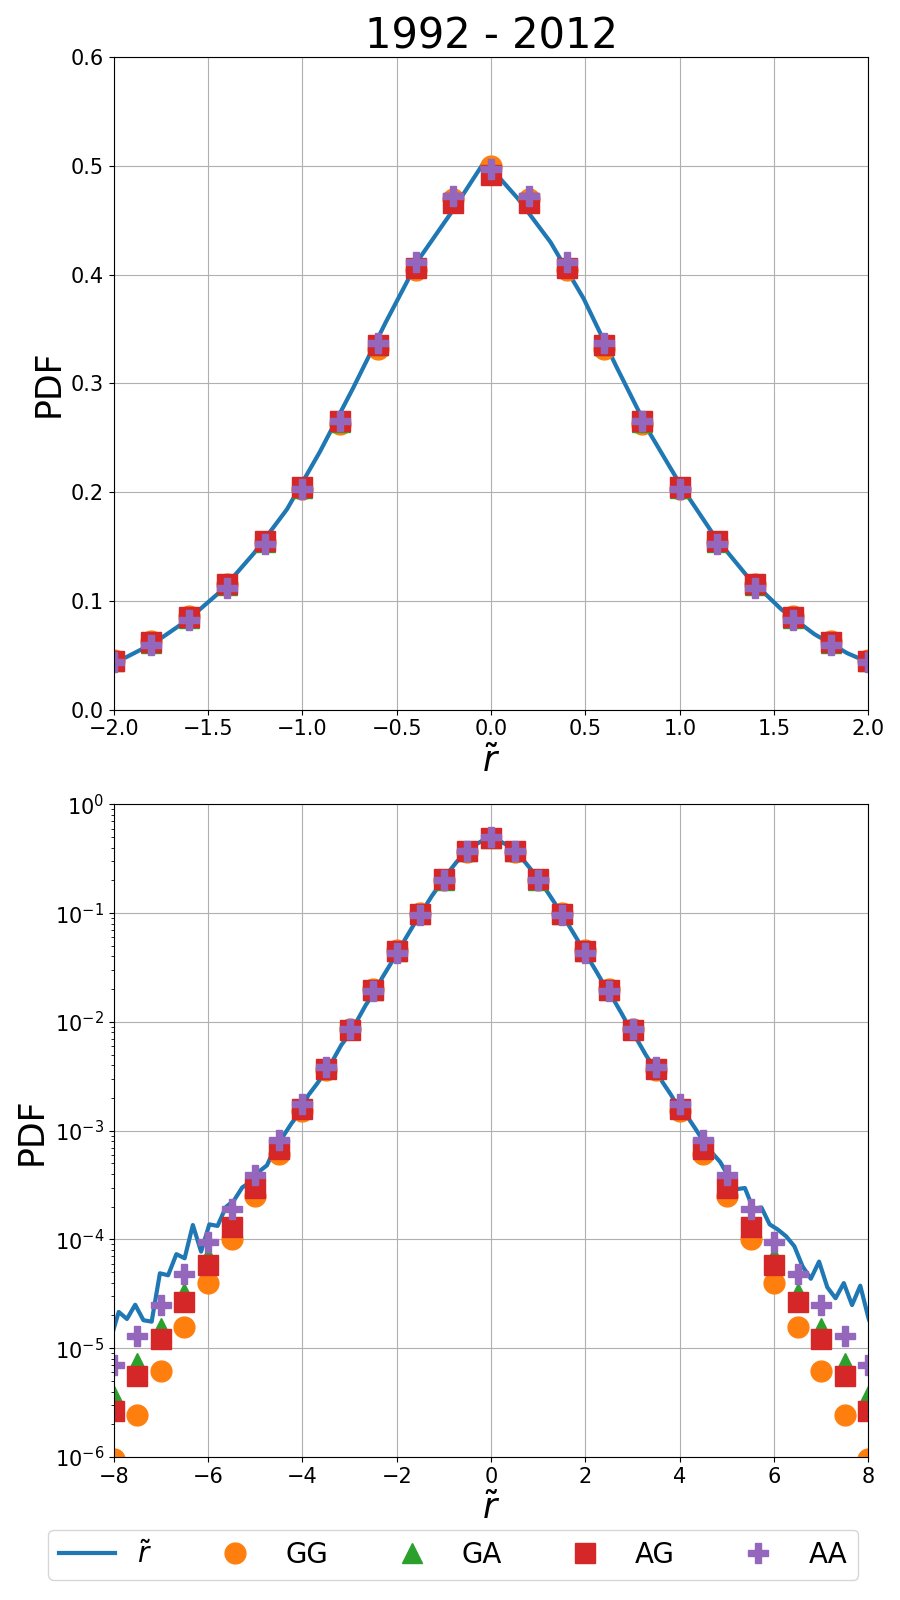
\includegraphics[width=\columnwidth]
    {figures/04_all_1992.png}
    \caption{}
    \label{fig:empirical_1992}
\end{figure}

\begin{figure}[htbp]
    \centering
    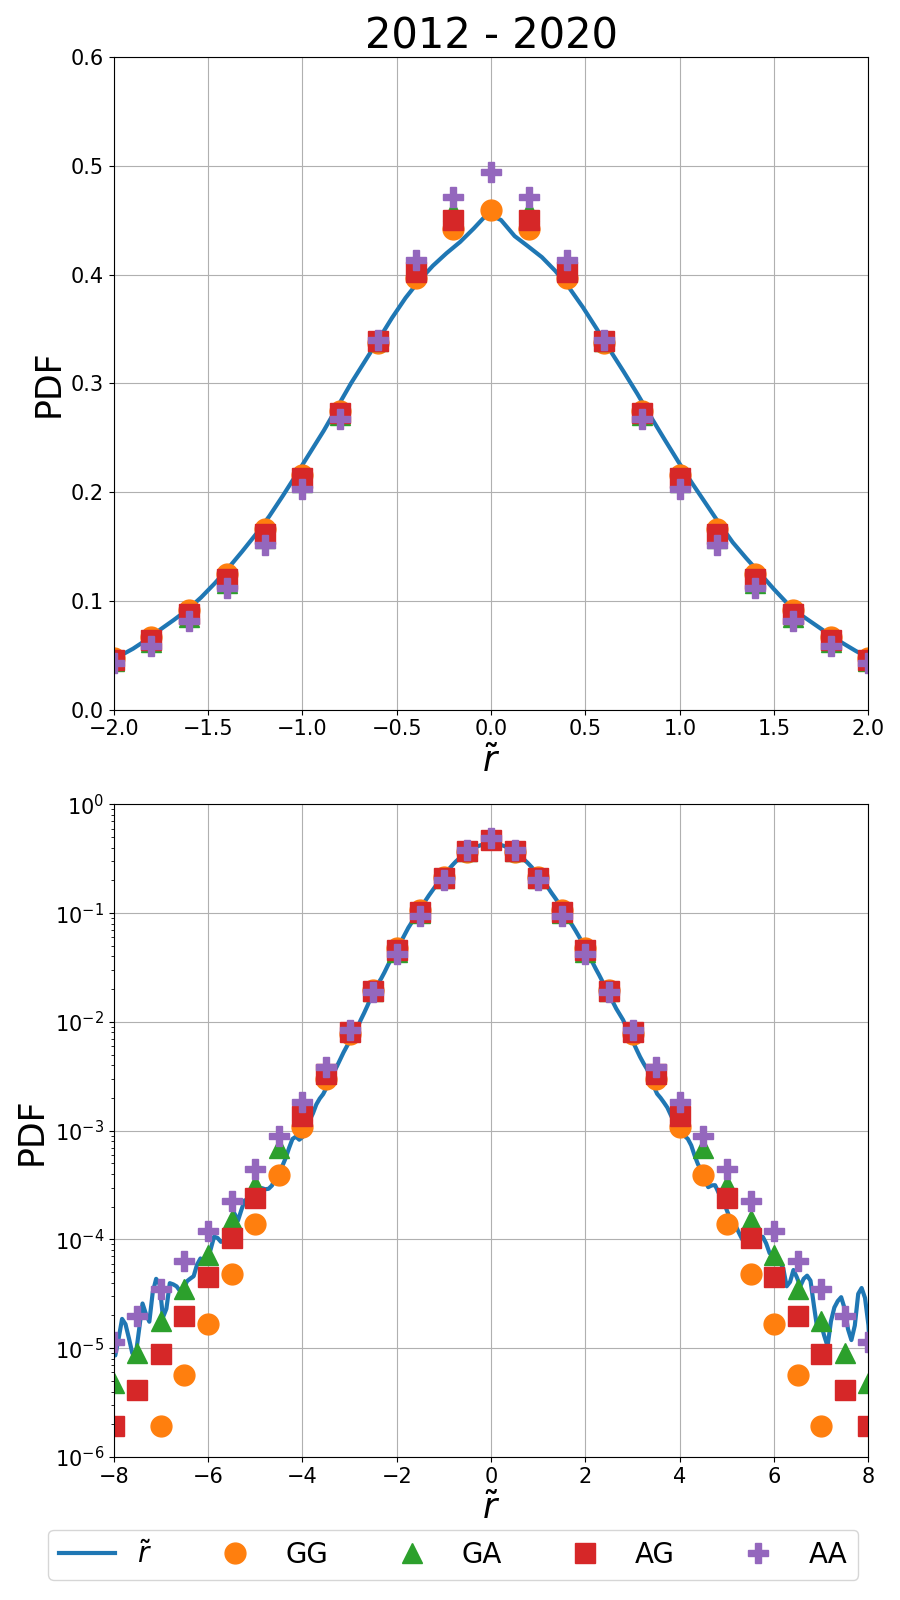
\includegraphics[width=\columnwidth]
    {figures/04_all_2012.png}
    \caption{}
    \label{fig:empirical_2012}
\end{figure}

%%%%%%%%%%%%%%%%%%%%%%%%%%%%%%%%%%%%%%%%%%%%%%%%%%%%%%%%%%%%%%%%%%%%%%%%%%%%%%%
\subsection{Response functions on physical time scale}
\label{subsec:response_function_physical}
